\documentclass{beamer}
\usepackage[utf8]{inputenc}
\usepackage{amsmath, pdfpages, pdflscape, lscape, color, listings, hyperref, amssymb, graphicx,textcomp,varioref, afterpage, subcaption, float, bm, tikz, multicol}

\global
\newcommand{\Fig}[1]{Figure \ref{#1}}
\newcommand{\fig}[1]{figure \ref{#1}}
\newcommand{\tab}[1]{table \ref{#1}}
\newcommand{\eq}[1]{equation \ref{#1}}
\newcommand{\Eq}[1]{Equation \ref{#1}}
\newcommand{\alg}[1]{algorithm \ref{#1}}
\newcommand{\Alg}[1]{Algorithm \ref{#1}}
\newcommand{\chp}[1]{chapter  \ref{#1}}
\newcommand{\Chp}[1]{Chapter  \ref{#1}}
\newcommand{\e}[1]{\cdot 10^{#1}}
\newcommand{\h}{\hbar}
\newcommand{\der}[2]{\frac{\partial #1}{\partial #2}}
\newcommand{\dder}[2]{\frac{\partial^2 #1}{\partial #2^2}}
\newcommand{\p}{\boldsymbol{P}}
\newcommand{\q}{\boldsymbol{q}}
\newcommand{\norm}[1]{\left\lVert#1\right\rVert}
\newcommand{\coef}[2]{\frac{\langle #1,#2\rangle_{\!Q}}{\norm{#2}^}}
\newcommand{\inner}[1]{\left\langle #1 \right\rangle_{\!Q}}

\newcommand{\E}[1]{\mbox{E}\!\left( #1 \right)}
\newcommand{\Var}[1]{\mbox{Var}\!\left( #1 \right)}

\newenvironment{test}[1]
{
 \usebackgroundtemplate{}
 \color{gray!30!black}
   \begin{tikzpicture}[remember picture, overlay]
     \node[anchor = center, opacity=.25] (image) at (current page.center) {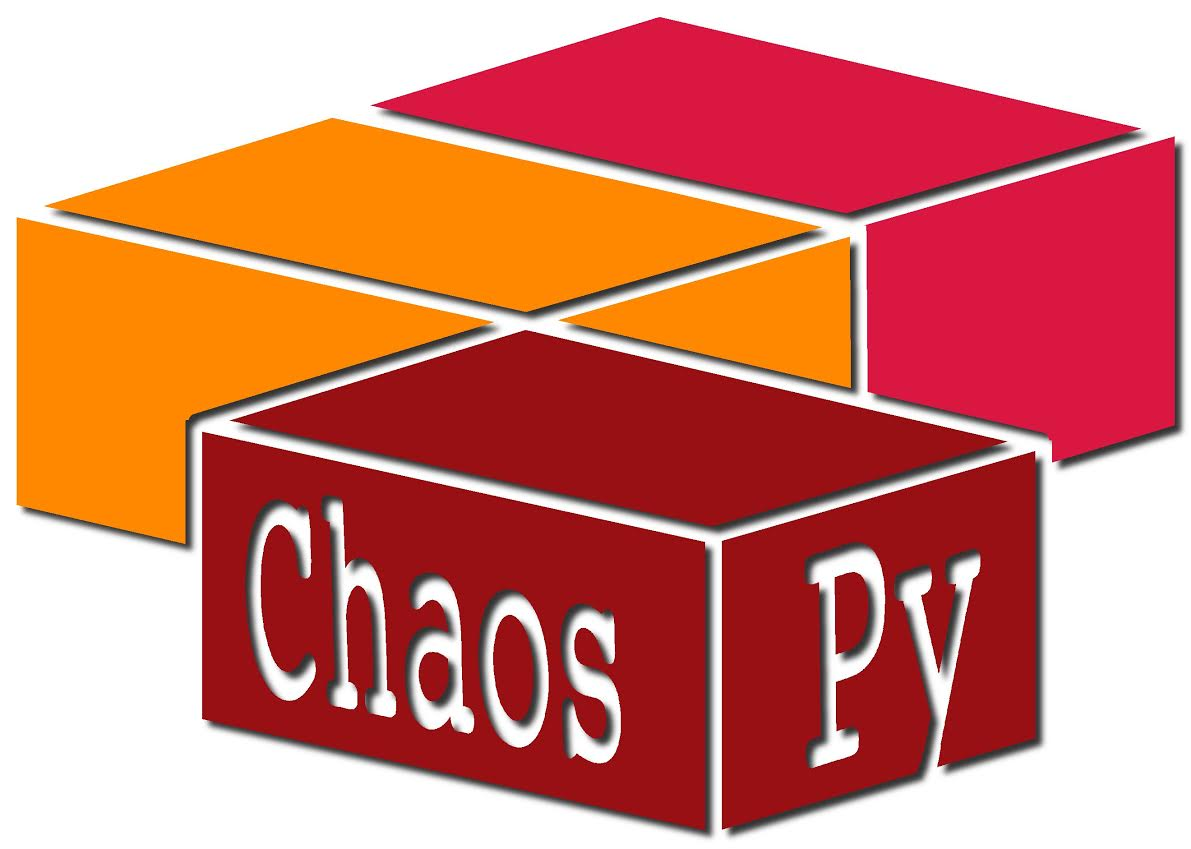
\includegraphics[scale=0.25]{chaospy_logo.jpg}};
   \end{tikzpicture}
 \begin{frame}[fragile,enviroment=chaospy]

}
{
 \end{frame}
}

 \lstset{
escapeinside={||},
basicstyle=\ttfamily\footnotesize,
columns=fixed
}


\newenvironment{chaospy}[1]
{\color{gray!30!black}
     \color{gray!30!black}
     \usebackgroundtemplate{
   \begin{tikzpicture}[remember picture, overlay]
     \node[anchor = center, opacity=.25] (image) at (current page.center) {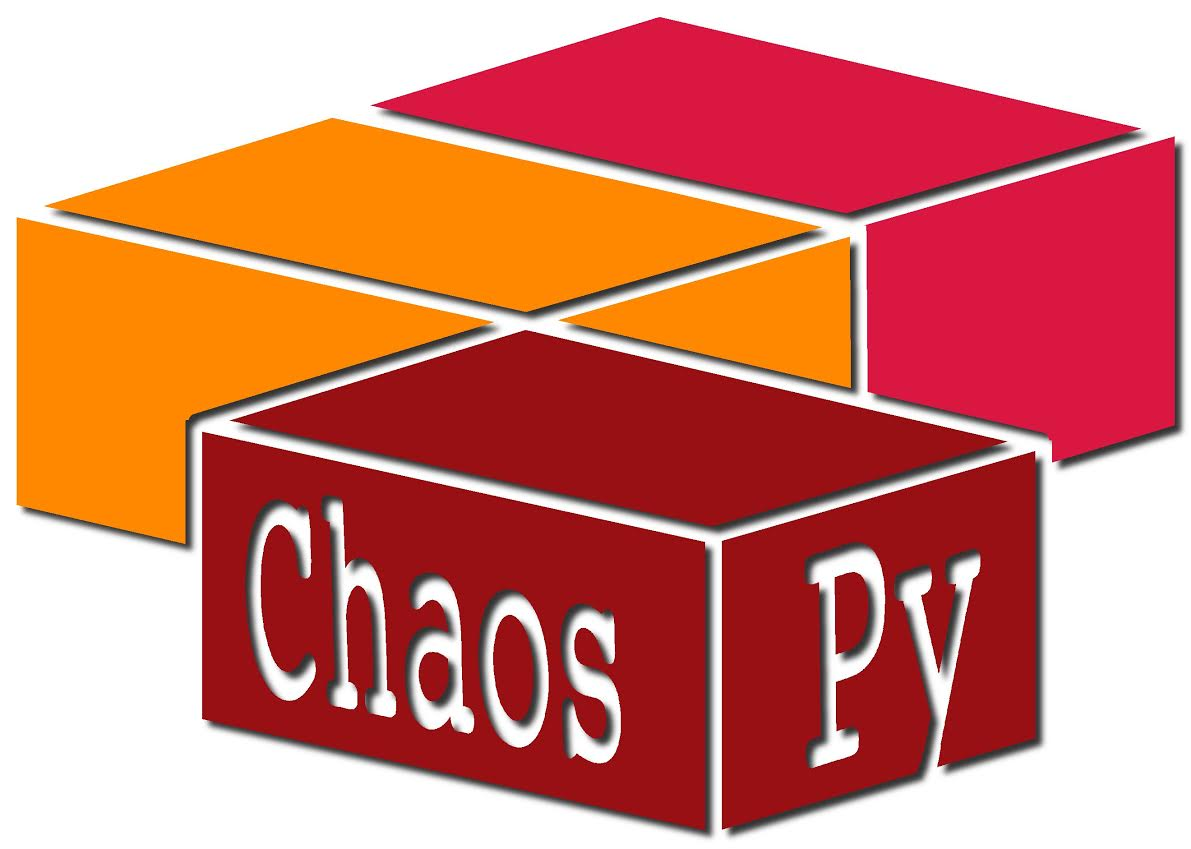
\includegraphics[scale=0.25]{chaospy_logo.jpg}};
   \end{tikzpicture}}
     \begin{frame}[fragile,environment=chaospy]
    \frametitle{{#1}}}
{\end{frame}}


\definecolor{keywords}{RGB}{255,0,90}
\definecolor{comments}{RGB}{0,0,113}
\definecolor{red}{RGB}{160,0,0}
\definecolor{green}{RGB}{0,150,0}

\usetheme{kalkulo}

\graphicspath{{./figures/}}


\title{Polynomial chaos expansions part 3: Intrusive Galerkin method}
\author{Jonathan Feinberg and Simen Tennøe}


\begin{document}



\begin{frame}
  \maketitle
\end{frame}



\begin{frame}[fragile]{Relevant links}
  \begin{center}
     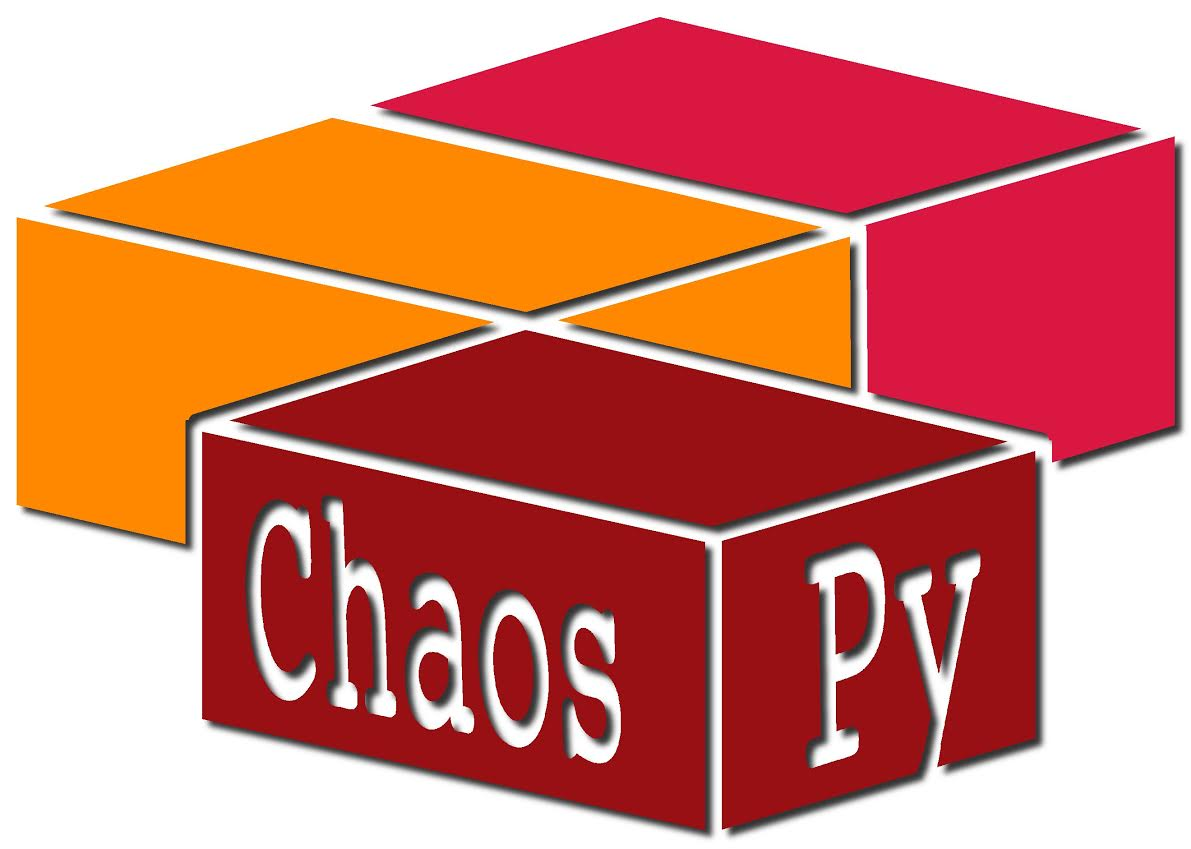
\includegraphics[width=.5\textwidth]{chaospy_logo.jpg}
  \end{center}
    \begin{alert}{A very basic introduction to scientific Python programming:}
    \scriptsize
      \href{http://hplgit.github.io/bumpy/doc/pub/sphinx-basics/index.html}{http://hplgit.github.io/bumpy/doc/pub/sphinx-basics/index.html}\\
%\verb;http://hplgit.github.io/bumpy/doc/pub/sphinx-basics/index.html;
  \end{alert}
  \begin{alert}{Installation instructions:}\\
  \scriptsize
      \href{https://github.com/hplgit/chaospy}{https://github.com/hplgit/chaospy}\\
%\verb;http://github.com/hplgit/chaospy/;
  \end{alert}
    \begin{alert}{Interactive sessions:}\\
  \scriptsize
\href{http://10.50.3.247:8888/}{http://10.50.3.247:8888/}

%\verb;http://10.50.3.247:8888/;
  \end{alert}
\end{frame}


\begin{frame}
 \frametitle{Repetition of our model problem}
  We have a simple differential equation
  \begin{align*}
    \frac{d u(x)}{dx} & =-au(x),\qquad u(0) = I
  \end{align*}
  \pause
  with the solution
  \[u(x) = Ie^{-ax}\]
  \pause
  with two random input variables:
   \[a \sim \text{Uniform(0, 0.1)}, \qquad I \sim \text{Uniform(8, 10)}\]
  Want to compute $\E{u}$ and $\Var{u}$
\end{frame}


\begin{frame}
 \frametitle{The Galerkin method is a projection method for approximating functions}

Given a function space $V$ and inner product on $V$ $\inner{u,v}=\int_0^Luvdx$

\begin{align*}
u'(x) &= g(x) \\
\int_0^L u'(x) v(x)dx &= \int_0^L g(x)v(x)dx,\quad\forall v\in V\\
\inner{u',v} &= \inner{g,v}\quad\mbox{(projection)}
\end{align*}

With $u(x; q) \approx \hat u_M(x; q) = \sum_{n=0}^N c_n(x) P_n(q)$ this leads to a linear system for
the coefficients $c_n$.
\end{frame}

\begin{frame}
 \frametitle{Calculating initial condition using Galerkin}
 \begin{align*}
 \hat u_M(0) &= I, & \hat u_M &= \sum_{n=0}^N c_n(x)P_n(q)\\
  \onslide<2-> {\sum_{n=0}^Nc_n(0)P_n &= I}\\
  \onslide<3-> {\inner{\sum_{n=0}^Nc_n(0)P_n,P_k} &= \inner{ I,P_k}
  & k&=0,\dots,N}\\
  \onslide<4-> {\sum_{n=0}^Nc_n(0)\inner{ P_n,P_k} &= \inner{ I,P_k} }\\
  \onslide<5-> {c_k(0)\inner{ P_k, P_k} &= \inner{ I,P_k} }\\
  \onslide<6-> {c_k(0) &= \frac{\inner{I, P_k}}{\inner{P_k, P_k}} = \frac{E(IP_k)}{E(P_k^2)}}\\
   \end{align*}

\end{frame}


\begin{frame}
 \frametitle{Galerkin applied to the differential equation}
%  \scriptsize
\footnotesize
 \begin{align*}
  \frac{d}{dx}\left(\hat u_M \right) &= -a \hat u_M\\
  \onslide<2-> {\frac{d}{dx}\left(\sum_{n=0}^Nc_nP_n \right) &= -a \sum_{n=0}^Nc_nP_n}\\
 \onslide<3-> {\inner{ \frac{d}{dx}\left(\sum_{n=0}^Nc_nP_n
 \right),P_k} &= \inner{-a \sum_{n=0}^Nc_nP_n,P_k} &
 k=0,\dots,N}\\
 \onslide<4-> {\frac{d}{dx}\sum_{n=0}^Nc_n\inner{ P_n ,P_k} &= -\sum_{n=0}^Nc_n\inner{ aP_n,P_k}}\\
 \onslide<5-> {\frac d{dx} c_k \inner{P_k, P_k}
 &= -\sum_{n=0}^N c_n \inner{aP_n, P_k} }\\
 \onslide<6-> {\frac{d}{dx}c_k
 &= -\sum_{n=0}^N c_n \frac{\inner{aP_n,P_k}}{\inner{P_k, P_k}}
 = -\sum_{n=0}^N c_n \frac{\E{aP_nP_k}}{\E{P_k^2}}}
 \end{align*}


\end{frame}



\begin{frame}
 \frametitle{The Galerkin Projection results in a coupled $(N+1)\times (N+1)$ system of differential equations}
 \begin{align*}
     \frac{d}{dx}c_k(x) &= -\sum_{n=0}^N c_n(x) \frac{E(aP_nP_k)}{E(P_k^2)}
     & k=0,\dots,N\\
 c_k(0) &= \frac{E(IP_k)}{E(P_k^2)}
 \end{align*}

\[ \frac{d}{dx}\bm{c} = -\bm{M}\bm{c},\quad M_{kn}= \frac{E(aP_nP_k)}{E(P_k^2)}\]
 \end{frame}


\begin{frame}
 \frametitle{The differential equation system is very sparse (mostly zeros)}
 \begin{columns}
     \column{.5\textwidth}
\begin{center}
    \begin{align*}
        E(P_nP_k)
    \end{align*}
  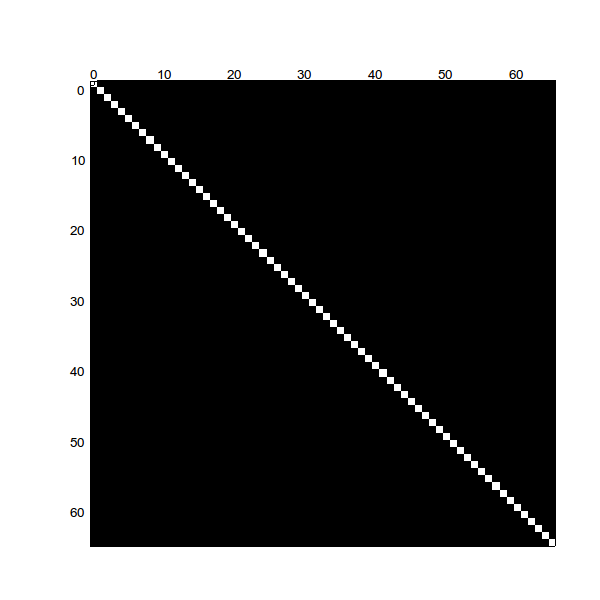
\includegraphics[width=0.9\textwidth]{binary_matrix1.png}
\end{center}
     \column{.5\textwidth}
     \begin{center}
    \begin{align*}
        E(aP_nP_k)
    \end{align*}
  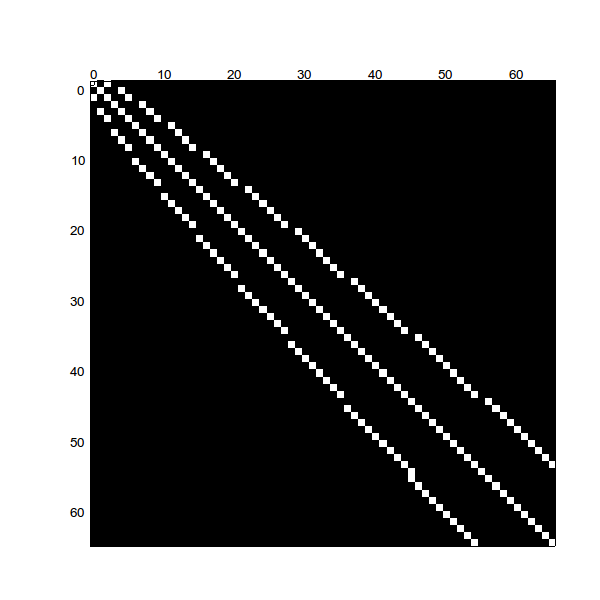
\includegraphics[width=0.9\textwidth]{binary_matrix.png}
     \end{center}
 \end{columns}
 \end{frame}

\begin{frame}
 \frametitle{Intrusive Galerkin usually converges faster}
\begin{itemize}[<+->]
\item Original problem: one scalar differential equation
\item Stochastic UQ problem: system of differential equations
\item The method is called \emph{intrusive Galerkin}
\item The original solver cannot be reused
\end{itemize}
\end{frame}

\begin{chaospy}{Solving the set of differential equations
    numerically}
    \scriptsize
\begin{lstlisting}[language=python]
import chaospy as cp
import numpy as np
import odespy
|\pause|
dist_a = cp.Uniform(0, 0.1)
dist_I = cp.Uniform(8, 10)
dist = cp.J(dist_a, dist_I) # joint multivariate dist
|\pause|
P, norms = cp.orth_ttr(n, dist, retall=True)|\pause|
variable_a, variable_I = cp.variable(2)
\end{lstlisting}
\end{chaospy}

\begin{chaospy}{Solving the set of differential equations numerically}
    \scriptsize
    \pause
\begin{lstlisting}[language=python]
PP = cp.outer(P, P)
E_aPP = cp.E(variable_a*PP, dist)
E_IP = cp.E(variable_I*P, dist)
|\pause|
def right_hand_side(c, x):            # c' = right_hand_side(c, x)
  return -np.dot(E_aPP, c)/norms    # -M*c

initial_condition = E_IP/norms
|\pause|
solver = odespy.RK4(right_hand_side)
solver.set_initial_condition(intitial_condition)
|\pause|
x = np.linspace(0, 10, 1000)
c = solver.solve(x)[0]
|\pause|
u_hat = cp.dot(P, c)
\end{lstlisting}
\end{chaospy}


\begin{frame}
 \frametitle{Intrusive Galerkin usually converges faster}
  \begin{figure}
  %\caption{Binary matrix of $E(aP_nP_k)$}
  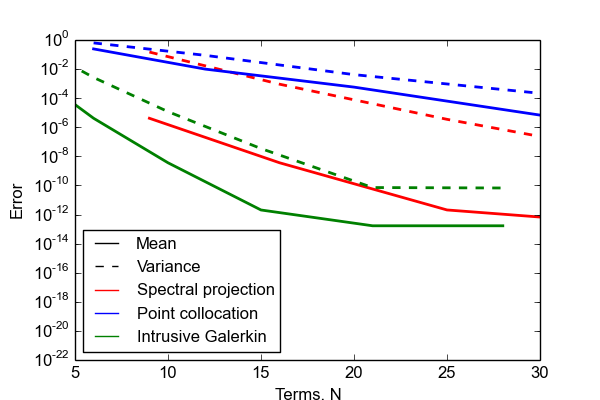
\includegraphics[width=0.85\textwidth]{convergence_gallerkin.png}
 \end{figure}
\end{frame}











\end{document}
